\chapter{Cylindrical Contact Homology in Dimension Three via Obstruction Bundle Gluing}
\label{b2}

\abstract{This lecture addresses the transversality issues associated with the moduli space of $J$-holomorphic curves. We specifically focus on cylindrical contact homology in the 3-dimensional case. The lecture will cover the resolution of transversality issues using obstruction bundle gluing techniques.}
\section{Compactification}

Let $\tilde{\mathcal{M}}(\gamma_+, \gamma_-): \left\{J\text{-holomorphic curves }\mathbb{R}\times S^1 \to \mathbb{R}\times M \right\}/\text{out of domain}$. There are asymptotic markers $\gamma_+$ and $\gamma_-$ on $\mathbb{R}\times M$, and at the points at $\infty$ of $\mathbb{R}\times S^1$ are markers in a way such that markers are mapped to markers. At each embedded Reeb orbit, choose a starting point. Define $\mathcal{M}=\tilde{\mathcal{M}}/\mathbb{R}$, which acts on $\mathbb{R}\times M$ by translation.

A sequence of $J$-holomorphic cylinder can converge to broken ones: we can break a cylinder $\mathbb{R}\times M$ into two cylinders $\mathbb{R}\times M$:

\begin{center}

\tikzset{every picture/.style={line width=0.75pt}} %set default line width to 0.75pt        

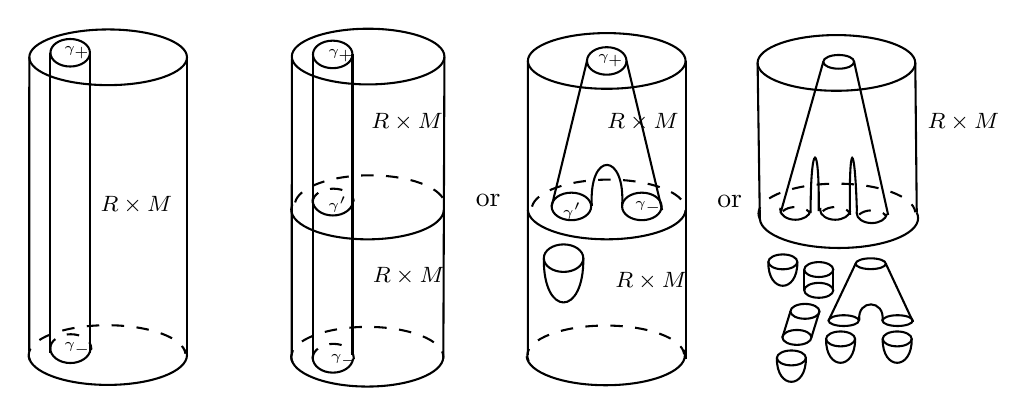
\begin{tikzpicture}[x=0.6pt,y=0.6pt,yscale=-1,xscale=1]
%uncomment if require: \path (0,300); %set diagram left start at 0, and has height of 300

%Shape: Ellipse [id:dp056395190934285244] 
\draw   (30.05,42.21) .. controls (30.05,32.95) and (51.31,25.44) .. (77.54,25.44) .. controls (103.76,25.44) and (125.02,32.95) .. (125.02,42.21) .. controls (125.02,51.48) and (103.76,58.98) .. (77.54,58.98) .. controls (51.31,58.98) and (30.05,51.48) .. (30.05,42.21) -- cycle ;
%Shape: Arc [id:dp6990177911205233] 
\draw  [draw opacity=0] (124.2,218.19) .. controls (124.74,219.28) and (125.02,220.4) .. (125.02,221.54) .. controls (125.02,231.47) and (103.68,239.51) .. (77.36,239.51) .. controls (51.54,239.51) and (30.52,231.77) .. (29.72,222.11) -- (77.36,221.54) -- cycle ; \draw   (124.2,218.19) .. controls (124.74,219.28) and (125.02,220.4) .. (125.02,221.54) .. controls (125.02,231.47) and (103.68,239.51) .. (77.36,239.51) .. controls (51.54,239.51) and (30.52,231.77) .. (29.72,222.11) ;  
%Straight Lines [id:da0017531833743447134] 
\draw    (30.05,41.97) -- (30.01,219.17) ;
%Straight Lines [id:da06191856902561077] 
\draw    (125.02,42.21) -- (125.02,221.93) ;
%Shape: Arc [id:dp7515744636820547] 
\draw  [draw opacity=0][dash pattern={on 4.5pt off 4.5pt}] (30.51,224.86) .. controls (29.98,223.78) and (29.7,222.67) .. (29.7,221.54) .. controls (29.7,211.61) and (50.85,203.57) .. (76.94,203.57) .. controls (102.32,203.57) and (123.02,211.19) .. (124.12,220.74) -- (76.94,221.54) -- cycle ; \draw  [dash pattern={on 4.5pt off 4.5pt}] (30.51,224.86) .. controls (29.98,223.78) and (29.7,222.67) .. (29.7,221.54) .. controls (29.7,211.61) and (50.85,203.57) .. (76.94,203.57) .. controls (102.32,203.57) and (123.02,211.19) .. (124.12,220.74) ;  
%Shape: Ellipse [id:dp170371749578063] 
\draw   (42.78,39.48) .. controls (42.78,34.9) and (48.11,31.19) .. (54.68,31.19) .. controls (61.25,31.19) and (66.58,34.9) .. (66.58,39.48) .. controls (66.58,44.06) and (61.25,47.77) .. (54.68,47.77) .. controls (48.11,47.77) and (42.78,44.06) .. (42.78,39.48) -- cycle ;
%Straight Lines [id:da7961683638948691] 
\draw    (42.78,39.48) -- (42.78,220.58) ;
%Straight Lines [id:da10134655093172151] 
\draw    (66.58,39.48) -- (66.58,220.58) ;
%Shape: Ellipse [id:dp0975147561159333] 
\draw   (188.15,41.77) .. controls (188.15,32.51) and (208.73,25) .. (234.11,25) .. controls (259.48,25) and (280.06,32.51) .. (280.06,41.77) .. controls (280.06,51.04) and (259.48,58.55) .. (234.11,58.55) .. controls (208.73,58.55) and (188.15,51.04) .. (188.15,41.77) -- cycle ;
%Shape: Arc [id:dp3077894307206215] 
\draw  [draw opacity=0] (279.39,222.94) .. controls (278.85,232.68) and (258.56,240.51) .. (233.6,240.51) .. controls (208.31,240.51) and (187.8,232.47) .. (187.8,222.54) .. controls (187.8,221.51) and (188.02,220.51) .. (188.44,219.53) -- (233.6,222.54) -- cycle ; \draw   (279.39,222.94) .. controls (278.85,232.68) and (258.56,240.51) .. (233.6,240.51) .. controls (208.31,240.51) and (187.8,232.47) .. (187.8,222.54) .. controls (187.8,221.51) and (188.02,220.51) .. (188.44,219.53) ;  
%Straight Lines [id:da4345493582140463] 
\draw    (188.15,42.97) -- (188.11,220.17) ;
%Straight Lines [id:da7275152931898132] 
\draw    (280.06,41.77) -- (279.4,223.71) ;
%Shape: Arc [id:dp15000914940586108] 
\draw  [draw opacity=0][dash pattern={on 4.5pt off 4.5pt}] (188.53,225.76) .. controls (188.05,224.72) and (187.8,223.64) .. (187.8,222.54) .. controls (187.8,212.61) and (208.3,204.57) .. (233.6,204.57) .. controls (258.89,204.57) and (279.39,212.61) .. (279.39,222.54) .. controls (279.39,222.67) and (279.39,222.8) .. (279.38,222.92) -- (233.6,222.54) -- cycle ; \draw  [dash pattern={on 4.5pt off 4.5pt}] (188.53,225.76) .. controls (188.05,224.72) and (187.8,223.64) .. (187.8,222.54) .. controls (187.8,212.61) and (208.3,204.57) .. (233.6,204.57) .. controls (258.89,204.57) and (279.39,212.61) .. (279.39,222.54) .. controls (279.39,222.67) and (279.39,222.8) .. (279.38,222.92) ;  
%Shape: Ellipse [id:dp7257031377511021] 
\draw   (200.88,40.48) .. controls (200.88,35.9) and (206.21,32.19) .. (212.78,32.19) .. controls (219.35,32.19) and (224.68,35.9) .. (224.68,40.48) .. controls (224.68,45.06) and (219.35,48.77) .. (212.78,48.77) .. controls (206.21,48.77) and (200.88,45.06) .. (200.88,40.48) -- cycle ;
%Straight Lines [id:da41430031772787657] 
\draw    (200.88,40.48) -- (200.88,221.58) ;
%Straight Lines [id:da8322496496190563] 
\draw    (224.68,40.48) -- (224.68,221.58) ;
%Shape: Arc [id:dp9948607311319655] 
\draw  [draw opacity=0] (279.72,134.27) .. controls (279.18,144.02) and (258.81,151.85) .. (233.76,151.85) .. controls (208.38,151.85) and (187.8,143.81) .. (187.8,133.88) .. controls (187.8,132.85) and (188.02,131.84) .. (188.45,130.86) -- (233.76,133.88) -- cycle ; \draw   (279.72,134.27) .. controls (279.18,144.02) and (258.81,151.85) .. (233.76,151.85) .. controls (208.38,151.85) and (187.8,143.81) .. (187.8,133.88) .. controls (187.8,132.85) and (188.02,131.84) .. (188.45,130.86) ;  
%Shape: Arc [id:dp47440163389587364] 
\draw  [draw opacity=0][dash pattern={on 4.5pt off 4.5pt}] (190.15,129.6) .. controls (192.26,120.45) and (211.6,113.29) .. (235.15,113.29) .. controls (260.12,113.29) and (280.35,121.34) .. (280.35,131.26) .. controls (280.35,132.27) and (280.14,133.26) .. (279.74,134.23) -- (235.15,131.26) -- cycle ; \draw  [dash pattern={on 4.5pt off 4.5pt}] (190.15,129.6) .. controls (192.26,120.45) and (211.6,113.29) .. (235.15,113.29) .. controls (260.12,113.29) and (280.35,121.34) .. (280.35,131.26) .. controls (280.35,132.27) and (280.14,133.26) .. (279.74,134.23) ;  
%Shape: Arc [id:dp6804839012339676] 
\draw  [draw opacity=0] (225.01,223.83) .. controls (224.48,228.48) and (219.25,232.13) .. (212.89,232.13) .. controls (206.17,232.13) and (200.72,228.07) .. (200.72,223.05) .. controls (200.72,222.56) and (200.77,222.07) .. (200.87,221.6) -- (212.89,223.05) -- cycle ; \draw   (225.01,223.83) .. controls (224.48,228.48) and (219.25,232.13) .. (212.89,232.13) .. controls (206.17,232.13) and (200.72,228.07) .. (200.72,223.05) .. controls (200.72,222.56) and (200.77,222.07) .. (200.87,221.6) ;  
%Shape: Arc [id:dp4500398352394417] 
\draw  [draw opacity=0][dash pattern={on 4.5pt off 4.5pt}] (200.83,224.21) .. controls (200.78,223.92) and (200.76,223.62) .. (200.76,223.33) .. controls (200.76,218.61) and (206.29,214.78) .. (213.11,214.78) .. controls (219.93,214.78) and (225.46,218.61) .. (225.46,223.33) .. controls (225.46,223.6) and (225.45,223.88) .. (225.41,224.15) -- (213.11,223.33) -- cycle ; \draw  [dash pattern={on 4.5pt off 4.5pt}] (200.83,224.21) .. controls (200.78,223.92) and (200.76,223.62) .. (200.76,223.33) .. controls (200.76,218.61) and (206.29,214.78) .. (213.11,214.78) .. controls (219.93,214.78) and (225.46,218.61) .. (225.46,223.33) .. controls (225.46,223.6) and (225.45,223.88) .. (225.41,224.15) ;  
%Shape: Arc [id:dp10273519473058612] 
\draw  [draw opacity=0] (224.88,126.86) .. controls (225,127.36) and (225.05,127.88) .. (225.05,128.4) .. controls (225.05,133.42) and (219.61,137.48) .. (212.89,137.48) .. controls (206.17,137.48) and (200.72,133.42) .. (200.72,128.4) .. controls (200.72,127.91) and (200.77,127.42) .. (200.87,126.95) -- (212.89,128.4) -- cycle ; \draw   (224.88,126.86) .. controls (225,127.36) and (225.05,127.88) .. (225.05,128.4) .. controls (225.05,133.42) and (219.61,137.48) .. (212.89,137.48) .. controls (206.17,137.48) and (200.72,133.42) .. (200.72,128.4) .. controls (200.72,127.91) and (200.77,127.42) .. (200.87,126.95) ;  
%Shape: Arc [id:dp9560702304930155] 
\draw  [draw opacity=0][dash pattern={on 4.5pt off 4.5pt}] (200.84,130.15) .. controls (200.79,129.87) and (200.76,129.57) .. (200.76,129.28) .. controls (200.76,124.89) and (206.29,121.33) .. (213.11,121.33) .. controls (219.82,121.33) and (225.28,124.77) .. (225.46,129.06) -- (213.11,129.28) -- cycle ; \draw  [dash pattern={on 4.5pt off 4.5pt}] (200.84,130.15) .. controls (200.79,129.87) and (200.76,129.57) .. (200.76,129.28) .. controls (200.76,124.89) and (206.29,121.33) .. (213.11,121.33) .. controls (219.82,121.33) and (225.28,124.77) .. (225.46,129.06) ;  
%Shape: Arc [id:dp7266228856012471] 
\draw  [draw opacity=0] (66.91,218.04) .. controls (66.38,222.69) and (61.16,226.34) .. (54.79,226.34) .. controls (48.07,226.34) and (42.62,222.27) .. (42.62,217.26) .. controls (42.62,216.76) and (42.67,216.28) .. (42.78,215.81) -- (54.79,217.26) -- cycle ; \draw   (66.91,218.04) .. controls (66.38,222.69) and (61.16,226.34) .. (54.79,226.34) .. controls (48.07,226.34) and (42.62,222.27) .. (42.62,217.26) .. controls (42.62,216.76) and (42.67,216.28) .. (42.78,215.81) ;  
%Shape: Arc [id:dp3689040331833249] 
\draw  [draw opacity=0][dash pattern={on 4.5pt off 4.5pt}] (42.73,218.41) .. controls (42.68,218.12) and (42.66,217.83) .. (42.66,217.53) .. controls (42.66,212.81) and (48.19,208.99) .. (55.01,208.99) .. controls (61.84,208.99) and (67.37,212.81) .. (67.37,217.53) .. controls (67.37,217.81) and (67.35,218.08) .. (67.31,218.35) -- (55.01,217.53) -- cycle ; \draw  [dash pattern={on 4.5pt off 4.5pt}] (42.73,218.41) .. controls (42.68,218.12) and (42.66,217.83) .. (42.66,217.53) .. controls (42.66,212.81) and (48.19,208.99) .. (55.01,208.99) .. controls (61.84,208.99) and (67.37,212.81) .. (67.37,217.53) .. controls (67.37,217.81) and (67.35,218.08) .. (67.31,218.35) ;  
%Shape: Ellipse [id:dp0661139858681199] 
\draw   (330.32,44.41) .. controls (330.32,35.15) and (351.58,27.64) .. (377.81,27.64) .. controls (404.03,27.64) and (425.29,35.15) .. (425.29,44.41) .. controls (425.29,53.67) and (404.03,61.18) .. (377.81,61.18) .. controls (351.58,61.18) and (330.32,53.67) .. (330.32,44.41) -- cycle ;
%Shape: Arc [id:dp8033107315109083] 
\draw  [draw opacity=0] (424.04,218.39) .. controls (424.58,219.47) and (424.87,220.59) .. (424.87,221.74) .. controls (424.87,231.66) and (403.53,239.71) .. (377.21,239.71) .. controls (351.39,239.71) and (330.36,231.97) .. (329.57,222.3) -- (377.21,221.74) -- cycle ; \draw   (424.04,218.39) .. controls (424.58,219.47) and (424.87,220.59) .. (424.87,221.74) .. controls (424.87,231.66) and (403.53,239.71) .. (377.21,239.71) .. controls (351.39,239.71) and (330.36,231.97) .. (329.57,222.3) ;  
%Straight Lines [id:da09066507708598825] 
\draw    (330.32,44.41) -- (330.28,221.6) ;
%Straight Lines [id:da3413965171016031] 
\draw    (425.29,44.41) -- (425.29,224.13) ;
%Shape: Arc [id:dp36547829111768615] 
\draw  [draw opacity=0][dash pattern={on 4.5pt off 4.5pt}] (330.78,225.06) .. controls (330.25,223.98) and (329.97,222.87) .. (329.97,221.74) .. controls (329.97,211.81) and (351.12,203.77) .. (377.21,203.77) .. controls (402.59,203.77) and (423.3,211.38) .. (424.39,220.94) -- (377.21,221.74) -- cycle ; \draw  [dash pattern={on 4.5pt off 4.5pt}] (330.78,225.06) .. controls (330.25,223.98) and (329.97,222.87) .. (329.97,221.74) .. controls (329.97,211.81) and (351.12,203.77) .. (377.21,203.77) .. controls (402.59,203.77) and (423.3,211.38) .. (424.39,220.94) ;  
%Shape: Ellipse [id:dp8629704518272938] 
\draw   (365.91,44.41) .. controls (365.91,39.83) and (371.24,36.12) .. (377.81,36.12) .. controls (384.38,36.12) and (389.71,39.83) .. (389.71,44.41) .. controls (389.71,48.99) and (384.38,52.7) .. (377.81,52.7) .. controls (371.24,52.7) and (365.91,48.99) .. (365.91,44.41) -- cycle ;
%Straight Lines [id:da8452678956957251] 
\draw    (365.91,44.41) -- (344.63,132.03) ;
%Straight Lines [id:da19999367359767395] 
\draw    (389.71,44.41) -- (411.17,134.3) ;
%Curve Lines [id:da16572232996503655] 
\draw    (368.81,131.66) .. controls (366.95,98.15) and (389.34,99.35) .. (387.05,132.03) ;
%Shape: Arc [id:dp6457528380286801] 
\draw  [draw opacity=0] (425.29,134.26) .. controls (424.72,144) and (403.68,151.83) .. (377.8,151.83) .. controls (351.71,151.83) and (330.53,143.87) .. (330.3,134.01) -- (377.8,133.85) -- cycle ; \draw   (425.29,134.26) .. controls (424.72,144) and (403.68,151.83) .. (377.8,151.83) .. controls (351.71,151.83) and (330.53,143.87) .. (330.3,134.01) ;  
%Shape: Arc [id:dp19216152259248287] 
\draw  [draw opacity=0][dash pattern={on 4.5pt off 4.5pt}] (332.81,132.15) .. controls (335.03,123.02) and (354.84,115.88) .. (378.95,115.88) .. controls (403.7,115.88) and (423.92,123.41) .. (425.23,132.88) -- (378.95,133.85) -- cycle ; \draw  [dash pattern={on 4.5pt off 4.5pt}] (332.81,132.15) .. controls (335.03,123.02) and (354.84,115.88) .. (378.95,115.88) .. controls (403.7,115.88) and (423.92,123.41) .. (425.23,132.88) ;  
%Shape: Ellipse [id:dp16448002790374439] 
\draw   (344.63,132.03) .. controls (344.63,127.45) and (349.95,123.74) .. (356.53,123.74) .. controls (363.1,123.74) and (368.43,127.45) .. (368.43,132.03) .. controls (368.43,136.61) and (363.1,140.32) .. (356.53,140.32) .. controls (349.95,140.32) and (344.63,136.61) .. (344.63,132.03) -- cycle ;
%Shape: Ellipse [id:dp9809662464110647] 
\draw   (387.05,132.03) .. controls (387.05,127.45) and (392.37,123.74) .. (398.94,123.74) .. controls (405.52,123.74) and (410.84,127.45) .. (410.84,132.03) .. controls (410.84,136.61) and (405.52,140.32) .. (398.94,140.32) .. controls (392.37,140.32) and (387.05,136.61) .. (387.05,132.03) -- cycle ;
%Shape: Ellipse [id:dp08366558813265468] 
\draw   (339.91,163.18) .. controls (339.91,158.6) and (345.24,154.89) .. (351.81,154.89) .. controls (358.39,154.89) and (363.71,158.6) .. (363.71,163.18) .. controls (363.71,167.76) and (358.39,171.47) .. (351.81,171.47) .. controls (345.24,171.47) and (339.91,167.76) .. (339.91,163.18) -- cycle ;
%Curve Lines [id:da09367632050515562] 
\draw    (339.91,163.18) .. controls (339.4,198.73) and (364.14,198.73) .. (363.71,163.18) ;
%Shape: Ellipse [id:dp8188508828087644] 
\draw   (468.66,45.61) .. controls (468.66,36.34) and (489.92,28.83) .. (516.14,28.83) .. controls (542.37,28.83) and (563.63,36.34) .. (563.63,45.61) .. controls (563.63,54.87) and (542.37,62.38) .. (516.14,62.38) .. controls (489.92,62.38) and (468.66,54.87) .. (468.66,45.61) -- cycle ;
%Shape: Arc [id:dp8117575286418532] 
\draw  [draw opacity=0] (564.51,135.73) .. controls (565.05,136.81) and (565.33,137.93) .. (565.33,139.08) .. controls (565.33,149) and (543.99,157.05) .. (517.67,157.05) .. controls (491.85,157.05) and (470.83,149.31) .. (470.04,139.64) -- (517.67,139.08) -- cycle ; \draw   (564.51,135.73) .. controls (565.05,136.81) and (565.33,137.93) .. (565.33,139.08) .. controls (565.33,149) and (543.99,157.05) .. (517.67,157.05) .. controls (491.85,157.05) and (470.83,149.31) .. (470.04,139.64) ;  
%Straight Lines [id:da331799661099899] 
\draw    (468.66,45.37) -- (470.01,139.6) ;
%Straight Lines [id:da9563297554519652] 
\draw    (563.63,45.61) -- (564.51,135.73) ;
%Shape: Arc [id:dp08014198609210887] 
\draw  [draw opacity=0][dash pattern={on 4.5pt off 4.5pt}] (470.01,139.6) .. controls (469.48,138.52) and (469.21,137.41) .. (469.21,136.28) .. controls (469.21,126.35) and (490.35,118.31) .. (516.44,118.31) .. controls (541.82,118.31) and (562.53,125.92) .. (563.63,135.48) -- (516.44,136.28) -- cycle ; \draw  [dash pattern={on 4.5pt off 4.5pt}] (470.01,139.6) .. controls (469.48,138.52) and (469.21,137.41) .. (469.21,136.28) .. controls (469.21,126.35) and (490.35,118.31) .. (516.44,118.31) .. controls (541.82,118.31) and (562.53,125.92) .. (563.63,135.48) ;  
%Shape: Ellipse [id:dp11318015897818423] 
\draw   (508.22,44.95) .. controls (508.22,42.66) and (512.38,40.81) .. (517.51,40.81) .. controls (522.64,40.81) and (526.8,42.66) .. (526.8,44.95) .. controls (526.8,47.24) and (522.64,49.09) .. (517.51,49.09) .. controls (512.38,49.09) and (508.22,47.24) .. (508.22,44.95) -- cycle ;
%Shape: Arc [id:dp5481702992712509] 
\draw  [draw opacity=0] (546.51,136.57) .. controls (546.06,139.65) and (542.17,142.05) .. (537.43,142.05) .. controls (532.39,142.05) and (528.31,139.34) .. (528.31,135.99) .. controls (528.31,135.62) and (528.36,135.25) .. (528.46,134.9) -- (537.43,135.99) -- cycle ; \draw   (546.51,136.57) .. controls (546.06,139.65) and (542.17,142.05) .. (537.43,142.05) .. controls (532.39,142.05) and (528.31,139.34) .. (528.31,135.99) .. controls (528.31,135.62) and (528.36,135.25) .. (528.46,134.9) ;  
%Shape: Arc [id:dp03984534439684717] 
\draw  [draw opacity=0][dash pattern={on 4.5pt off 4.5pt}] (529.88,136.9) .. controls (531.49,135.39) and (534.33,134.38) .. (537.57,134.38) .. controls (541.2,134.38) and (544.33,135.64) .. (545.79,137.47) -- (537.57,139.78) -- cycle ; \draw  [dash pattern={on 4.5pt off 4.5pt}] (529.88,136.9) .. controls (531.49,135.39) and (534.33,134.38) .. (537.57,134.38) .. controls (541.2,134.38) and (544.33,135.64) .. (545.79,137.47) ;  
%Straight Lines [id:da3617949510353735] 
\draw    (508.22,44.95) -- (482.46,136.1) ;
%Straight Lines [id:da649340590604436] 
\draw    (526.8,44.95) -- (547.3,137.17) ;
%Curve Lines [id:da8727790296078328] 
\draw    (500.59,136) .. controls (500.55,91.73) and (506.07,91.73) .. (505.46,134.9) ;
%Curve Lines [id:da4875409262510293] 
\draw    (524.3,137.17) .. controls (523.55,91.73) and (527.23,91.73) .. (528.46,134.9) ;
%Shape: Ellipse [id:dp7111828464384535] 
\draw   (475.13,165.41) .. controls (475.13,162.93) and (479.04,160.93) .. (483.87,160.93) .. controls (488.7,160.93) and (492.61,162.93) .. (492.61,165.41) .. controls (492.61,167.89) and (488.7,169.89) .. (483.87,169.89) .. controls (479.04,169.89) and (475.13,167.89) .. (475.13,165.41) -- cycle ;
%Curve Lines [id:da9672709945361355] 
\draw    (475.13,165.41) .. controls (474.75,184.63) and (492.92,184.63) .. (492.61,165.41) ;
%Shape: Ellipse [id:dp8770495266103071] 
\draw   (496.76,170.05) .. controls (496.76,167.57) and (500.67,165.56) .. (505.5,165.56) .. controls (510.33,165.56) and (514.24,167.57) .. (514.24,170.05) .. controls (514.24,172.52) and (510.33,174.53) .. (505.5,174.53) .. controls (500.67,174.53) and (496.76,172.52) .. (496.76,170.05) -- cycle ;
%Shape: Ellipse [id:dp4700005658957731] 
\draw   (496.76,182.56) .. controls (496.76,180.08) and (500.67,178.07) .. (505.5,178.07) .. controls (510.33,178.07) and (514.24,180.08) .. (514.24,182.56) .. controls (514.24,185.03) and (510.33,187.04) .. (505.5,187.04) .. controls (500.67,187.04) and (496.76,185.03) .. (496.76,182.56) -- cycle ;
%Shape: Ellipse [id:dp3742015758632733] 
\draw   (488.45,195.21) .. controls (488.45,192.74) and (492.36,190.73) .. (497.19,190.73) .. controls (502.01,190.73) and (505.93,192.74) .. (505.93,195.21) .. controls (505.93,197.69) and (502.01,199.69) .. (497.19,199.69) .. controls (492.36,199.69) and (488.45,197.69) .. (488.45,195.21) -- cycle ;
%Shape: Ellipse [id:dp05712935955362908] 
\draw   (483.6,210.9) .. controls (483.6,208.43) and (487.51,206.42) .. (492.34,206.42) .. controls (497.16,206.42) and (501.08,208.43) .. (501.08,210.9) .. controls (501.08,213.38) and (497.16,215.39) .. (492.34,215.39) .. controls (487.51,215.39) and (483.6,213.38) .. (483.6,210.9) -- cycle ;
%Straight Lines [id:da2384391731418305] 
\draw    (496.76,170.05) -- (496.76,182.56) ;
%Straight Lines [id:da33392656495348927] 
\draw    (514.24,170.05) -- (514.24,182.56) ;
%Straight Lines [id:da566045394847106] 
\draw    (505.93,195.21) -- (501.08,210.9) ;
%Straight Lines [id:da5614446278591068] 
\draw    (488.45,195.21) -- (483.6,210.9) ;
%Shape: Ellipse [id:dp035227786182282506] 
\draw   (480.27,223.26) .. controls (480.27,220.78) and (484.18,218.77) .. (489.01,218.77) .. controls (493.84,218.77) and (497.75,220.78) .. (497.75,223.26) .. controls (497.75,225.73) and (493.84,227.74) .. (489.01,227.74) .. controls (484.18,227.74) and (480.27,225.73) .. (480.27,223.26) -- cycle ;
%Curve Lines [id:da7379429542962657] 
\draw    (480.27,223.26) .. controls (479.89,242.47) and (498.06,242.47) .. (497.75,223.26) ;
%Shape: Ellipse [id:dp5542296065150325] 
\draw   (509.9,211.8) .. controls (509.9,209.33) and (513.82,207.32) .. (518.64,207.32) .. controls (523.47,207.32) and (527.38,209.33) .. (527.38,211.8) .. controls (527.38,214.28) and (523.47,216.29) .. (518.64,216.29) .. controls (513.82,216.29) and (509.9,214.28) .. (509.9,211.8) -- cycle ;
%Curve Lines [id:da7423459609744811] 
\draw    (509.9,211.8) .. controls (509.53,231.02) and (527.7,231.02) .. (527.38,211.8) ;
%Shape: Ellipse [id:dp24342029029087775] 
\draw   (544,211.8) .. controls (544,209.33) and (547.91,207.32) .. (552.74,207.32) .. controls (557.56,207.32) and (561.48,209.33) .. (561.48,211.8) .. controls (561.48,214.28) and (557.56,216.29) .. (552.74,216.29) .. controls (547.91,216.29) and (544,214.28) .. (544,211.8) -- cycle ;
%Curve Lines [id:da21595115366288664] 
\draw    (544,211.8) .. controls (543.62,231.02) and (561.79,231.02) .. (561.48,211.8) ;
%Shape: Ellipse [id:dp9507589820584572] 
\draw   (527.68,166.53) .. controls (527.68,164.74) and (531.76,163.28) .. (536.79,163.28) .. controls (541.82,163.28) and (545.9,164.74) .. (545.9,166.53) .. controls (545.9,168.32) and (541.82,169.77) .. (536.79,169.77) .. controls (531.76,169.77) and (527.68,168.32) .. (527.68,166.53) -- cycle ;
%Straight Lines [id:da7901347005685313] 
\draw    (527.68,166.53) -- (511.39,200.8) ;
%Straight Lines [id:da056288864133154926] 
\draw    (545.9,166.53) -- (562.33,201.69) ;
%Curve Lines [id:da988145377883118] 
\draw    (529.9,200.65) .. controls (528.48,187.55) and (545.61,188.02) .. (543.86,200.8) ;
%Shape: Ellipse [id:dp23604569535188302] 
\draw   (511.39,200.8) .. controls (511.39,199.01) and (515.47,197.55) .. (520.5,197.55) .. controls (525.53,197.55) and (529.61,199.01) .. (529.61,200.8) .. controls (529.61,202.59) and (525.53,204.04) .. (520.5,204.04) .. controls (515.47,204.04) and (511.39,202.59) .. (511.39,200.8) -- cycle ;
%Shape: Ellipse [id:dp7261778653447537] 
\draw   (543.86,200.8) .. controls (543.86,199.01) and (547.94,197.55) .. (552.97,197.55) .. controls (558,197.55) and (562.08,199.01) .. (562.08,200.8) .. controls (562.08,202.59) and (558,204.04) .. (552.97,204.04) .. controls (547.94,204.04) and (543.86,202.59) .. (543.86,200.8) -- cycle ;
%Shape: Arc [id:dp3746223374313047] 
\draw  [draw opacity=0] (524.51,134.57) .. controls (524.06,137.65) and (520.17,140.05) .. (515.43,140.05) .. controls (510.39,140.05) and (506.31,137.34) .. (506.31,133.99) .. controls (506.31,133.62) and (506.36,133.25) .. (506.46,132.9) -- (515.43,133.99) -- cycle ; \draw   (524.51,134.57) .. controls (524.06,137.65) and (520.17,140.05) .. (515.43,140.05) .. controls (510.39,140.05) and (506.31,137.34) .. (506.31,133.99) .. controls (506.31,133.62) and (506.36,133.25) .. (506.46,132.9) ;  
%Shape: Arc [id:dp21450518339030733] 
\draw  [draw opacity=0][dash pattern={on 4.5pt off 4.5pt}] (507.88,134.9) .. controls (509.49,133.39) and (512.33,132.38) .. (515.57,132.38) .. controls (519.2,132.38) and (522.33,133.64) .. (523.79,135.47) -- (515.57,137.78) -- cycle ; \draw  [dash pattern={on 4.5pt off 4.5pt}] (507.88,134.9) .. controls (509.49,133.39) and (512.33,132.38) .. (515.57,132.38) .. controls (519.2,132.38) and (522.33,133.64) .. (523.79,135.47) ;  
%Shape: Arc [id:dp37481817018727304] 
\draw  [draw opacity=0] (500.51,134.57) .. controls (500.06,137.65) and (496.17,140.05) .. (491.43,140.05) .. controls (486.39,140.05) and (482.31,137.34) .. (482.31,133.99) .. controls (482.31,133.62) and (482.36,133.25) .. (482.46,132.9) -- (491.43,133.99) -- cycle ; \draw   (500.51,134.57) .. controls (500.06,137.65) and (496.17,140.05) .. (491.43,140.05) .. controls (486.39,140.05) and (482.31,137.34) .. (482.31,133.99) .. controls (482.31,133.62) and (482.36,133.25) .. (482.46,132.9) ;  
%Shape: Arc [id:dp03724951552805966] 
\draw  [draw opacity=0][dash pattern={on 4.5pt off 4.5pt}] (483.88,134.9) .. controls (485.49,133.39) and (488.33,132.38) .. (491.57,132.38) .. controls (495.2,132.38) and (498.33,133.64) .. (499.79,135.47) -- (491.57,137.78) -- cycle ; \draw  [dash pattern={on 4.5pt off 4.5pt}] (483.88,134.9) .. controls (485.49,133.39) and (488.33,132.38) .. (491.57,132.38) .. controls (495.2,132.38) and (498.33,133.64) .. (499.79,135.47) ;  

% Text Node
\draw (139.08,121.83) node [anchor=north west][inner sep=0.75pt]    {$\rightsquigarrow $};
% Text Node
\draw (71.12,123.83) node [anchor=north west][inner sep=0.75pt]  [font=\footnotesize]  {$\mathbb{R} \times M$};
% Text Node
\draw (208.07,35.68) node [anchor=north west][inner sep=0.75pt]  [font=\tiny]  {$\gamma _{+}$};
% Text Node
\draw (49.15,212.24) node [anchor=north west][inner sep=0.75pt]  [font=\tiny]  {$\gamma _{-}$};
% Text Node
\draw (209.61,219.23) node [anchor=north west][inner sep=0.75pt]  [font=\tiny]  {$\gamma _{-}$};
% Text Node
\draw (208.07,124.24) node [anchor=north west][inner sep=0.75pt]  [font=\tiny]  {$\gamma '$};
% Text Node
\draw (297.07,122.73) node [anchor=north west][inner sep=0.75pt]   [align=left] {or};
% Text Node
\draw (49.15,33.72) node [anchor=north west][inner sep=0.75pt]  [font=\tiny]  {$\gamma _{+}$};
% Text Node
\draw (392.94,127.04) node [anchor=north west][inner sep=0.75pt]  [font=\tiny]  {$\gamma _{-}$};
% Text Node
\draw (349.35,128.14) node [anchor=north west][inner sep=0.75pt]  [font=\tiny]  {$\gamma '$};
% Text Node
\draw (370.56,38.38) node [anchor=north west][inner sep=0.75pt]  [font=\tiny]  {$\gamma _{+}$};
% Text Node
\draw (442.53,123.33) node [anchor=north west][inner sep=0.75pt]   [align=left] {or};
% Text Node
\draw (235.12,166.83) node [anchor=north west][inner sep=0.75pt]  [font=\footnotesize]  {$\mathbb{R} \times M$};
% Text Node
\draw (234.12,73.83) node [anchor=north west][inner sep=0.75pt]  [font=\footnotesize]  {$\mathbb{R} \times M$};
% Text Node
\draw (376.12,73.83) node [anchor=north west][inner sep=0.75pt]  [font=\footnotesize]  {$\mathbb{R} \times M$};
% Text Node
\draw (381.12,169.83) node [anchor=north west][inner sep=0.75pt]  [font=\footnotesize]  {$\mathbb{R} \times M$};
% Text Node
\draw (569.12,73.83) node [anchor=north west][inner sep=0.75pt]  [font=\footnotesize]  {$\mathbb{R} \times M$};


\end{tikzpicture}

\end{center}

where for the rightmost diagram, each of the bottom components is a map to $\mathbb{R}^n$.

\begin{definition}

Let $(F,j)$ be a Riemann surface, $\dot{F}=F$ a finite subset, and $u:(\dot{F},j)\stackrel{J-\text{holomorphic}}{\to} (\mathbb{R}\times M, J)$. Then the \textbf{Hofer energy} is
\[
E(u)=\sup_{\phi \in \mathcal{C}} \int_{\dot{F}} u^* d(\phi, \alpha)
\]
where
\[
\mathcal{C} = \left\{ \phi: \mathbb{R} \to [1,2] \mid
\begin{cases}
\phi(s) = 1 & \text{if } s \ll 0, \\
\phi(s) = 2 & \text{if } s \gg 0, \\
\phi'(s) \ge 0 & \text{for all } s \in \mathbb{R}
\end{cases}
\right\}
\]

\end{definition}

\begin{proposition}

\begin{align*}
E(u)&= 2\sum_{i=1}^{k_+} \mathcal{A}(\gamma_{+,i})-\sum_{i=1}^{k_-} \mathcal{A}(\gamma_{-,i}) \\
&\ge 0.
\end{align*}

\end{proposition}

\section{Grading}

\begin{theorem}

If $u: (\dot{E}, j)\to \mathbb{R}\times M$ is $J$-holomorphic, the following are equivalent:
\begin{itemize}
\item $E(u)<\infty$
\item For any puncture $p$ of $\dot{F}$, either $p$ is removable or $u$ converges to some Reeb orbit along $P$.
\end{itemize}

\end{theorem}

Assume the $H_1(M; \mathbb{Z})$ is torsion free. If $H_1(M)=0$, then for each Reeb orbit $\gamma$, fix a surface $F_\gamma \subset M$ spanning $\gamma$. If $H_1(M; \mathbb{Z})\neq 0$, choose a basis of $H_1(M)$ and represent it by oriented curves $c_1,...c_k$. Choose a trivialization of $\xi/c_1$. For any Reeb orbit $\gamma$, choose $F_\gamma$ such that $[\partial F_\gamma]=[\gamma]-\sum n_i [c_i]$. Choose a trivialization of $\xi \mid_{\gamma}$ so that it extends over $F_\gamma$ and agrees with the trivialization of $\xi/c_i$. This defines a Conley-Zehder index for each $\gamma$.

For each $J$-holomorphic cylinder $u$, we can attach $F_{\gamma_+}$ and $F_{\gamma_-}$:
\begin{center}
\tikzset{every picture/.style={line width=0.75pt}} %set default line width to 0.75pt        

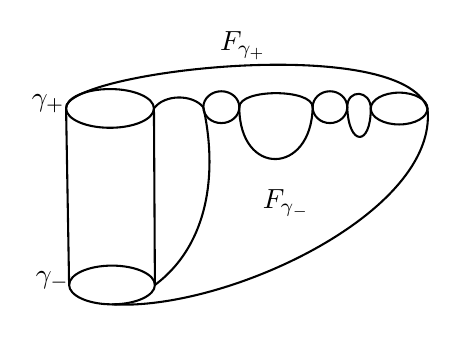
\begin{tikzpicture}[x=0.5pt,y=0.5pt,yscale=-1,xscale=1]
%uncomment if require: \path (0,300); %set diagram left start at 0, and has height of 300

%Shape: Ellipse [id:dp8909013950100437] 
\draw   (85,82) .. controls (85,74.27) and (99.21,68) .. (116.75,68) .. controls (134.29,68) and (148.5,74.27) .. (148.5,82) .. controls (148.5,89.73) and (134.29,96) .. (116.75,96) .. controls (99.21,96) and (85,89.73) .. (85,82) -- cycle ;
%Straight Lines [id:da939999364801372] 
\draw    (85,82) -- (87.2,209.6) ;
%Straight Lines [id:da32030547024849] 
\draw    (148.5,82) -- (149.2,209.6) ;
%Shape: Ellipse [id:dp22593738557210807] 
\draw   (87.2,209.6) .. controls (87.2,201.87) and (101.08,195.6) .. (118.2,195.6) .. controls (135.32,195.6) and (149.2,201.87) .. (149.2,209.6) .. controls (149.2,217.33) and (135.32,223.6) .. (118.2,223.6) .. controls (101.08,223.6) and (87.2,217.33) .. (87.2,209.6) -- cycle ;
%Shape: Ellipse [id:dp3903650035201627] 
\draw   (184.2,81.1) .. controls (184.2,74.75) and (190.02,69.6) .. (197.2,69.6) .. controls (204.38,69.6) and (210.2,74.75) .. (210.2,81.1) .. controls (210.2,87.45) and (204.38,92.6) .. (197.2,92.6) .. controls (190.02,92.6) and (184.2,87.45) .. (184.2,81.1) -- cycle ;
%Shape: Ellipse [id:dp439043297167095] 
\draw   (263.2,81.1) .. controls (263.2,74.75) and (268.8,69.6) .. (275.7,69.6) .. controls (282.6,69.6) and (288.2,74.75) .. (288.2,81.1) .. controls (288.2,87.45) and (282.6,92.6) .. (275.7,92.6) .. controls (268.8,92.6) and (263.2,87.45) .. (263.2,81.1) -- cycle ;
%Shape: Ellipse [id:dp5515211986371753] 
\draw   (305.2,82.1) .. controls (305.2,75.75) and (314.38,70.6) .. (325.7,70.6) .. controls (337.02,70.6) and (346.2,75.75) .. (346.2,82.1) .. controls (346.2,88.45) and (337.02,93.6) .. (325.7,93.6) .. controls (314.38,93.6) and (305.2,88.45) .. (305.2,82.1) -- cycle ;
%Curve Lines [id:da43171084391564163] 
\draw    (118.2,223.6) .. controls (201.2,228.6) and (354.2,156.6) .. (346.2,82.1) ;
%Curve Lines [id:da12535479193092525] 
\draw    (85,82) .. controls (82.2,55.6) and (327.2,26.6) .. (346.2,82.1) ;
%Curve Lines [id:da515259067066461] 
\draw    (288.2,81.1) .. controls (289.2,109.6) and (305.2,109.6) .. (305.2,82.1) ;
%Curve Lines [id:da3208943864453322] 
\draw    (210.2,81.1) .. controls (210.2,131.6) and (262.2,130.6) .. (263.2,81.1) ;
%Curve Lines [id:da7762191468457265] 
\draw    (210.2,81.1) .. controls (210.2,67.6) and (263.2,67.6) .. (263.2,81.1) ;
%Curve Lines [id:da23187615015116236] 
\draw    (288.2,81.1) .. controls (288.2,67.6) and (305.2,68.6) .. (305.2,82.1) ;
%Curve Lines [id:da3836381595978182] 
\draw    (148.5,82) .. controls (156.2,71.6) and (176.2,71.6) .. (184.2,81.1) ;
%Curve Lines [id:da3396096780840039] 
\draw    (149.2,209.6) .. controls (189.2,179.6) and (194.2,126.6) .. (184.2,81.1) ;

% Text Node
\draw (58,69.4) node [anchor=north west][inner sep=0.75pt]    {$\gamma _{+}$};
% Text Node
\draw (61,197.4) node [anchor=north west][inner sep=0.75pt]    {$\gamma _{-}$};
% Text Node
\draw (194,24.4) node [anchor=north west][inner sep=0.75pt]    {$F_{\gamma _{+}}$};
% Text Node
\draw (225,138.4) node [anchor=north west][inner sep=0.75pt]    {$F_{\gamma _{-}}$};

\end{tikzpicture}
\end{center}

which gives an element in $H_2(M)$.

Assume does not exist a contractible Reeb orbits. We define a chain complex $(C_*, \partial)$ where $C_*$ is a free $\mathbb{Q}[H_2(M)]$ module generated by all good Reeb orbits. For each $A\in H_2(M)$, $| A|  = -2 \langle c_1(\xi), A \rangle$, define $\partial_{\gamma_+}= \sum_{\gamma_-, A}\# \mathcal{M}(\gamma_+, \gamma_-, A) e^A \frac{1}{m(\gamma_-)}\gamma_-$ where $m(\gamma_-)$ is the multiplcity of $\gamma_-$. This gives $|\gamma_+| -| \gamma_- | -| A| =1$. Define $| \gamma| =\mu_{c_2}(\gamma)+n-3$.

\begin{definition}

$\gamma$ is \textbf{bad} if $\gamma$ is multiple cover of embedded $\gamma'$ and $\mu_{\text{cz}}(\gamma)-\mu_{\text{cz}}(\gamma')$ is odd.

\end{definition}

\begin{example}

For $\dim \mathcal{M}=3$, $\gamma$ is bad if and only if $\gamma$ is an even multiple cover of a negative hyperbolic one.

\end{example}

If there exists a contractible Reeb orbits:
\vspace{-20pt}
\begin{figure}[htbp]
  \centering
  \includegraphics[width=1\textwidth]{images/bao1.png}
  \label{fig:bi14}
\end{figure}
\vspace{-40pt} % Adjust this value to control the space

This gives the contact homology. One important variant of the contact homology is the (rational) symplectic field theory.

\begin{example}

In $\dim =3$, if $\gamma$ is hyperbolic, then
\[
\mu_{\text{cz}}(\gamma, k) = k \mu_{\text{cz}}(\gamma).
\]

Let $u$ be $J$-holomorphic. If $\text{ind }u = \mu(\gamma_+)-\mu(\gamma)-| A| $. If $u$ is $k$-fold cover of $u'$ and there are no elliptic orbits, then $\text{ind }u = k\cdot \text{ind }u'$.

If $u'$ transverses $\text{ind}$ and $\text{ind } u' \ge 1$, then $\text{ind }u \ge k$. In the definition of $\partial, \text{ind }(u)=1 \implies k=1$.

We can always eliminate elliptic orbits up to any action:
\begin{center}
    
\tikzset{every picture/.style={line width=0.75pt}} %set default line width to 0.75pt        

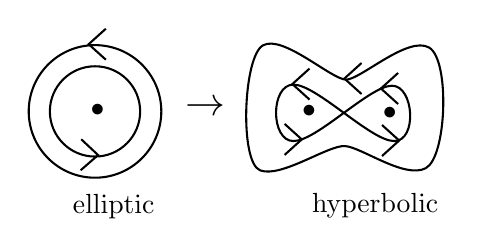
\begin{tikzpicture}[x=0.4pt,y=0.4pt,yscale=-1,xscale=1]
%uncomment if require: \path (0,300); %set diagram left start at 0, and has height of 300

%Shape: Circle [id:dp08144944578189617] 
\draw   (70.82,119.71) .. controls (70.82,86.63) and (97.63,59.82) .. (130.71,59.82) .. controls (163.79,59.82) and (190.6,86.63) .. (190.6,119.71) .. controls (190.6,152.79) and (163.79,179.6) .. (130.71,179.6) .. controls (97.63,179.6) and (70.82,152.79) .. (70.82,119.71) -- cycle ;
%Shape: Circle [id:dp39773554712775216] 
\draw   (89.93,119.71) .. controls (89.93,97.19) and (108.19,78.93) .. (130.71,78.93) .. controls (153.23,78.93) and (171.49,97.19) .. (171.49,119.71) .. controls (171.49,142.23) and (153.23,160.49) .. (130.71,160.49) .. controls (108.19,160.49) and (89.93,142.23) .. (89.93,119.71) -- cycle ;
%Shape: Polygon Curved [id:ds02793189593737866] 
\draw   (399,96.5) .. controls (419,96.5) and (422,146.5) .. (401,146.5) .. controls (380,146.5) and (331,95.5) .. (310,95.5) .. controls (289,95.5) and (289,146.5) .. (310,146.5) .. controls (331,146.5) and (379,96.5) .. (399,96.5) -- cycle ;
%Shape: Polygon Curved [id:ds03073014229495996] 
\draw   (357.5,91) .. controls (370.5,91) and (413.5,51) .. (432.5,62) .. controls (451.5,73) and (448.5,161) .. (429.5,171) .. controls (410.5,181) and (371.5,152) .. (356.5,151) .. controls (341.5,150) and (299,180) .. (280,173) .. controls (261,166) and (264.5,70) .. (282.5,60) .. controls (300.5,50) and (344.5,91) .. (357.5,91) -- cycle ;
\draw   (371.5,104) -- (356,90) -- (371.5,76) ;
\draw   (324.5,109) -- (309,95) -- (324.5,81) ;
\draw   (390,132) -- (405.5,146) -- (390,160) ;
\draw   (302,131) -- (317.5,145) -- (302,159) ;
\draw   (404.5,113) -- (389,99) -- (404.5,85) ;
\draw   (140.5,73) -- (125,59) -- (140.5,45) ;
\draw   (118.25,144.87) -- (133.5,159.14) -- (117.76,172.86) ;

% Text Node
\draw (124,110.4) node [anchor=north west][inner sep=0.75pt]    {$\bullet $};
% Text Node
\draw (315,111.4) node [anchor=north west][inner sep=0.75pt]    {$\bullet $};
% Text Node
\draw (388,113.4) node [anchor=north west][inner sep=0.75pt]    {$\bullet $};
% Text Node
\draw (210,107.4) node [anchor=north west][inner sep=0.75pt]  [font=\Large]  {$\rightarrow $};
% Text Node
\draw (108,192) node [anchor=north west][inner sep=0.75pt]   [align=left] {elliptic};
% Text Node
\draw (324,191) node [anchor=north west][inner sep=0.75pt]   [align=left] {hyperbolic};

\end{tikzpicture}

\end{center}

These two images have the same contact structure, but different contact forms.

\end{example}